%% The following is a directive for TeXShop to indicate the main file
%%!TEX root = diss.tex

\chapter{Implementations and Evaluations}
\label{ch:Implementations}

In this chapter we evaluate the four metadata augmentation algorithms with the City of Surrey's Open Data\footnote{https://www.surrey.ca/services-payments/online-services/open-data}. We first discuss the procedure of retrieving, preprocessing, and preparing data, and outline some techniques commonly used for dealing with large quantities of data. We also discuss the external knowledge bases and the trained parameters for our algorithms. We then describe how we selected the testing set from Surrey Open Data, and how we manually created a gold standard set, which allows us to discuss in detail how we evaluate the algorithms using the testing set and the gold standard. Due to the lack of existing literature that evaluates metadata generation for tabular data, we invent our own metrics in our evaluation. We are limited to very simple metrics that are yet to be validated on realistic scenarios. We state a number of assumptions that we make in order to achieve acceptable performance.

The discussion of the results of our evaluation follows, where we show that the tables found and the tags augmented have a high recall without sacrificing too much precision. Finally, we propose more realistic evaluation metrics that allow us to relax our assumptions but require the availability of human expertise.

%%%%%%%%%%%%%%%%%%%%%%%%%%%%%%%%%%%%%%%%%%%%%%%%%%%%%%%%%%%%%%%%%%%%%%
\section{Retrieving Surrey open data}
\label{sec:RetrievingSurreyOpenData}

The City of Surrey offers an open data catalogue online, where the resources can be downloaded manually from a URL or programmatically. Each resource has a category and a list of tags. The open data catalogue offers functionalities for browsing, filtering by tags and categories, and searching by keyword. Users can browse each resource by clicking on the link to each resource.

Filtering by specific categories or specific tags allows the user to narrow down the resources they want to see. The keyword search functionality permits the user to enter keywords in a search box, and the search engine looks for the keywords in the resources metadata. Due to the order of actions performed by the user, it is possible that a user misses many resources that should appear in the results. For example, if the user filters by category first, examines the results, and then further filters by specific tags, then resources in other categories will not be displayed in the results even if they contain some specific tags.

The resources and the metadata can be located using unique URLs, which one can visit to download the resources and the metadata. The resources are stored using a portal named Comprehensive Knowledge Archive Network (CKAN), the data can be accessed via an API request with the GET command and a parameter specifying the name of the dataset. The metadata for each resource is stored separately on a directory named ArcGIS REST Services Directory. Each resource's metadata is accessed via an API request with the GET command and a parameter specifying the format (JSON or PJSON) of the metadata. We wrote a script to download the resources and metadata programmatically.

Each resource stores data instances in multiple formats, which includes PDF, JSON, CSV, KML, etc. For example, the data instances in PDF are reports created by the city council, and the data instances in KML are geographic data representing points on a map. In our study, we only retrieved data instances in JSON or CSV because they are easier to process. We give a higher priority to data instances in CSV format, because JSON and CSV data instances store similar data. It is possible to change the data instances in JSON format to CSV when a resource does not contain a CSV format of the data. We parsed the JSON data and transformed the data to CSV in the following manner: the key in the JSON data becomes the header of a column and the value becomes one of the column values. If the value is a JSON object instead of a string, then these JSON data instances are dropped because we cannot transform the data to CSV. All data instances are converted to CSV format, and stored in Python's Pandas DataFrame as input to our algorithm implementations.

If the data instance or metadata is hierarchical (such as JSON or XML), we assume the hierarchical data is well-formed.

\subsection{Preprocessing data}

We discuss the preprocessing of table data and metadata before we perform metadata augmentation. We first give a unique name to each data instance, which is also used to identify the metadata of the data instance. We save all the metadata in one place, which includes the schema and the tags. This allows us to easily modify them and make comparisons among them. During the initialization step, we collect all the unique tags from all tables, and compute the distance (using N-gram) between each pair of tags. We can reuse these distance values while performing table search. We also collect all the attributes of a data instance.

We semantically enrich the attributes and tags by collecting all the metadata of the table for every attribute or tag, and we extract nouns from the metadata by using the tagger functions in the NLTK library \cite{loper-bird-2002-nltk} available as a software package. These taggers are pretrained. We extract nouns from the \textit{table name, category, table description, tags}, and \textit{header row} (as shown in \autoref{fig:example-parks}), and let every noun except the word that we want to enrich become the context of the word. We then use the NLTK's WordNet database to retrieve the word senses and example sentences, and extract the nouns in a similar manner to create the context of a word. Comparing a word sense context and a metadata context is done by computing the set difference between the two bags of words. We then attach the Synset to the attribute or tag word once word sense disambiguation is performed, and the result of the semantic enrichment is saved.

We note that all of the above is made possible because of the availability of metadata. Since open data are typically physical collections with metadata that contains enough information \cite{Rahm2016Case} such as attributes, title, description, and tags, it is generally easy for us to work with open data and to generate more metadata.

During schema matching, we construct a matching matrix, where the rows are items (attributes or tags) from the first set and the columns are the items (attributes or tags) from the second set. The matrix stores the similarity values of item pairs, and we use this matrix to find pairs to create correspondences. We also save this matrix because our algorithm may make the same comparisons in a future iteration.

We have downloaded a FastText skip-gram model containing pre-trained word vectors \cite{mikolov-etal-2018-advances}, which predicts surrounding words from a given word, and computes distance between words.

%%%%%%%%%%%%%%%%%%%%%%%%%%%%%%%%%%%%%%%%%%%%%%%%%%%%%%%%%%%%%%%%%%%%%%
\section{Tuning parameters in algorithms}
\label{sec:TuningParametersInAlgorithms}

An issue that we would like to raise for schema matching is that for each matching criteria, the decision threshold is usually chosen by hand, and the empirical choice may not be the best. We will leave tuning of the threshold using supervised learning as future work.

A user is required to manually set a value for each of the parameters in our algorithms. The abstraction of a tuning knob for each of the parameters is proposed in \cite{books/sp/bellahsene11}, where each parameter is restricted to a range of values, and the value is increased or decreased until optimality is reached. Without tuning these parameters, we are unable to obtain the desired performance. The parameters that we tuned manually include the decision thresholds used in schema matching and the weights for each matching criteria in hybrid matching. In order for our model to be generalized, such that we are able to solve a problem using an existing model given some new data, the thresholds and weights need to be tuned using supervised learning \cite{Duchateau2009YAM,Doan2001Reconciling}. In the schema matching problem, data from one domain and a small set of ground truth correspondences are provided as input, and the parameters are adjusted based on how accurate the matching is compared to the ground truth. In order to describe the interaction between the data and the model independent of the domain, the work in \cite{Pham2016Semantic} trained semantic labelers using training data from one data domain (soccer), and showed that the parameters can be reused in semantic labelers of a different data domain (museum). Even though the data are from different domains, the labelers use domain-independent characteristics of the data such as the histogram similarity and the distribution similarity. We intend to leverage these characteristics as future work.

\subsection{User-guided schema matching}

Fully-automated schema matching does not perform well, since a schema matching algorithm typically uses parameters that require tuning \cite{books/sp/bellahsene11}. Parameters include thresholds and weights. Users can guide schema matching by setting the parameters before schema matching is performed. The parameters can also be tuned automatically by using external knowledge, such as training the hybrid matching weights and thresholds using pre-existing correspondences created by hand \cite{Ehrig2004QOM}. The version of hybrid matching we implemented in \autoref{sec:DataDrivenApproach} relies on training the weights from pre-existing correspondences. The user can also guide schema matching by providing feedback at the end of the schema matching algorithm by correcting wrong correspondences. In \cite{Duchateau2009YAM}, schema matching is made interactive, where a candidate match is presented to the user, and the user provides corrections to wrong correspondences. Corrections of the parameters are then made according to feedback to improve the accuracy of future schema matchings.

Without data experts, the interactive schema matching approach cannot be adopted. Instead, we guide schema matching by providing one table as the base table, and use this table to find related tables.

%%%%%%%%%%%%%%%%%%%%%%%%%%%%%%%%%%%%%%%%%%%%%%%%%%%%%%%%%%%%%%%%%%%%%%
\section{Evaluations}
\label{sec:Evaluations}

There are three types of experiments for evaluating a system: offline evaluation without user interaction, limited-scope user studies, and online evaluation while the system is used by many users. We only perform offline evaluation and leave additional experiments as future work. We first describe how we select the test data for our evaluations. We then introduce how a gold standard helps us in offline evaluations, and describe how we create the gold standard. We next outline our design of evaluating the augmented metadata with the gold standard. The four metadata augmentation algorithms are evaluated with the gold standard. We discuss the results of our experiments and analyze the different algorithms.

\subsection{Test data selection}
\label{ssec:TestDataSelection}

The data instances in Surrey Open Data are grouped into different sets by the category metadata. A number of tables from each domain is selected into the test set. Tables that do not have at least 5 columns are omitted. Similarly, tables lacking the schema or sufficient metadata to create the contexts are also omitted. To evaluate our implementations, we created a test plan consisting of different tests. Each test uses a different set of data as the repository, and they differ in the set size. The repository of each test uses $k$ data instances, where $k$ = 5 or 10, and one of the data instances is the base table.

Of the $k$ data instances in the repository, a proportion of the data instances is related to the base table, and the remaining are not related. For example, when $k$ = 5 and $Parks$ is the base table, we choose 2 tables in the \textit{Parks} data domain and 2 tables in another domain, which produces the set \{\textit{Parks}, \textit{ParkSpecimenTrees}, \textit{ParkScreenTrees}, \textit{DrainageCatchBasins}, and \textit{WaterDykeInfrastructure}\}. Alternatively, we can choose all 4 tables from the \textit{Parks} domain, or all 4 tables from another domain. In our study, $Parks$ is the only base table we chose, but as future work we intend to choose tables from other domains as the base table.

\subsection{Gold standard}
\label{ssec:GoldStandard}

The gold standard set we created consists of a list of tags for each table. We use the tags to compare with the algorithm's output tags. The gold standard set for Surrey Open Data contains augmented tags for 90 tables spanning 5 data domains (based on 5 $categories$ in the metadata). We manually collected around 700 tags in the Surrey Open Data repository, which makes up the vocabulary of the tags. %We explain why it make sense to evaluate the output tags against the gold standard. 
We worked on the data for more than a year, and have good knowledge of what data are in the repository and thus were in a reasonable position to create the gold standard ourselves. 
%We also have contacting information of the data authors, so that we can contact them to clarify if we cannot understand some data. 
However, we would like our gold standard to be validated by the data experts as future work, by providing them with the vocabulary of around 700 topics and the augmented metadata tags we created for each table. Once they provide us with their feedback, we can make changes to our gold standard set. In the case that the number of tags is much larger than 700, we would need to consider crowd-sourcing the gold standard.

We also have guidelines for creating the list of augmented topics in the gold standard. Our goal is to try to reduce bias. Bias is present when we have augmented too many tags in one data domain, but missed many tags in another domain. This bias is common because data are collected based on human decisions, and people tend to only collect data from sources they are familiar with or they have access to.

The guidelines we give below aim to reduce bias in the gold standard we create. We manually collect tags from each table into a set, and cluster the tags (using N-gram as the distance function) to find groups of similar tags. We then examine each table one by one, while having access to the 700 tags, the clusters of tags, and all tables in the same domain. For existing tags $L_{s}$ of the table $s$, we find the cluster $\textit{Cluster}(L_{sj})$ each tag $L_{sj}$ is in. For each candidate tag $L_{si}$, we retrieve all tables $S_{j}$ already containing tag $L_{sj}$, and inspect the data and the metadata of each table $s'$ in $S_{j}$ to decide whether the candidate tag $L_{sj}$ should be added. We also inspect each table $s'$ containing the tag $L_{sj}$ and discover additional similar tags $L_{s'}$ that could be added to the gold standard of $L_{s}$. We built a user-interactive tool that assists us to perform all of the above. %We did not have full confidence that the gold standard is correct, but we modified the gold standard while evaluating the output tags. 
We added any tags that we missed and we removed tags that seemed incorrect after each test run. We did not count these test runs as part of the accuracy calculation.

\subsection{Comparing output augmented tags with gold standard}
\label{ssec:ComparingOutputAugmentedTagsWithGoldStandard}

After tables are augmented with tags using our algorithms, we measure the accuracy on the gold standard we created. To evaluate a given test set on the gold standard, we tailor the gold standard such that it only contains tables in the test set. Given a test set, we show an example of the gold standard compared with the output augmented tags. Let the base table be Parks, and let the repository contain the tables  \{\textit{Parks}, \textit{ParkSpecimenTrees}, \textit{DrainageCatchBasins}, \textit{ParkScreenTrees}\}. The gold standard for this particular test should only contain tables related to Parks. For this test, the augmented tags for tables \{\textit{Parks}, \textit{ParkSpecimenTrees}, \textit{ParkScreenTrees}\} are in the gold standard.

Each of the tables in the gold standard contains a set of augmented tags. Let the augmented tags of the \textit{Parks} table contain [\textit{environment}, \textit{green}, \textit{nature}, \textit{parks}, \textit{trees}] in the gold standard. Its original tags are [\textit{environment}, \textit{green}, \textit{nature}, \textit{parks}]. Similarly, the augmented tags of \textit{ParkSpecimenTrees} are [\textit{environment}, \textit{green}, \textit{nature}, \textit{parks}, \textit{trees}] and the augmented tags of \textit{ParkScreenTrees} are [\textit{environment}, \textit{green}, \textit{nature}, \textit{parks}, \textit{trees}]. As future work, we would like to tailor each table in the gold standard to be specific for a test, where the only tags contained are the ones shared between the tables in the test set. For a table in the gold standard, any tags shared with a table not in the test set should not be included in the gold standard. For example, \textit{Parks} is augmented with a tag \textit{bike} which is only present in \textit{GreenInfrastructureNetwork}, but since \textit{GreenInfrastructureNetwork} is not in the test set, the gold standard should not include this tag. Currently we do not enforce this restriction.

The output of metadata augmentation is a set of tables and the augmented topics of each table. We compare this output with the tailored gold standard. We measure in terms of precision and recall. The precision of a test is:
\[
\frac{\text{number of correct tables}}{\text{number of tables found by search}^{2}}\sum\limits _{\text{table found by search}}\frac{\text{correctly augmented tags}}{\text{all augmented tags for table}}
\]

Similarly, the recall of a test is:
\[
\frac{\text{number of correct tables}}{\text{number of tables in gold standard}^{2}}\sum\limits _{\text{table in gold standard}}\frac{\text{correctly augmented tags}}{\text{all augmented tags for table}}
\]

In general, we identify output tags that should not belong in certain tables as incorrect in the computation for precision. We identify gold standard tags missing in certain tables as incorrect in the computation for recall.

We show an example of comparing the augmented tags with the tailored gold standard. An algorithm produces [\textit{environment},\textit{green},\textit{nature},\textit{parks},\textit{trees}] for \textit{Parks}, [\textit{environment}, \textit{green}, \textit{parks}, \textit{trees}] for \textit{ParkSpecimenTrees}, and [\textit{devices}, \textit{drainage}, \textit{infrastructure}] for \textit{DrainageCatchBasins} as the output. Using the gold standard in \autoref{ssec:GoldStandard}, the precision is $(2/3^{2})*(5/5+4/4+0/3)$. Only 2 of the 3 tables are correctly retrieved by search, and all tags in the retrieved tables are correct. The recall is $(2/3^{2})*(5/5 + 4/5 + 0/5)$. Only 2 of the 3 retrieved tables are in the gold standard, and 9 of the 15 tags are in the gold standard. Note that \textit{DrainageCatchBasins} is in the output but not in the gold standard, and so the computation for precision takes this extra table into account but not for recall.

In addition to precision and recall, we compute the F-measure, which is based on both precision and recall. The F-measure is commonly used in measuring information retrieval accuracy and natural language processing problems. We use the F1 score for the F-measure of a test, given by:
\[
\ensuremath{F_{1}}=2\ensuremath{\cdot}\frac{\text{precision}\cdot\text{recall}}{\text{precision}+\text{recall}}
\]

The F1 score gives us a sense of the overall ability of our algorithms to augment tags.

\begin{figure}
    \centering
    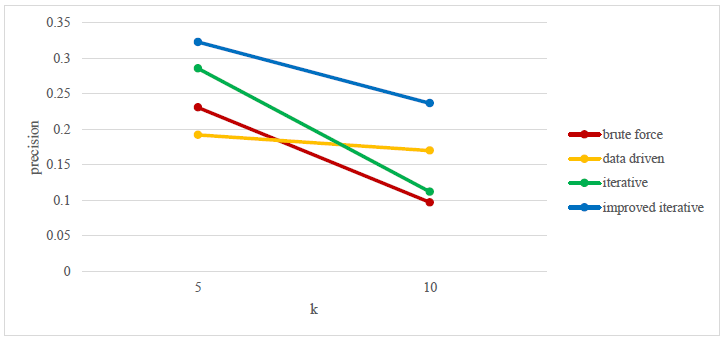
\includegraphics[width=5in]{figures/precision-different-algorithms.png}
    \caption{Precision of augmented tags for different algorithms}
    \label{fig:precision-different-algorithms}
\end{figure}

\begin{figure}
    \centering
    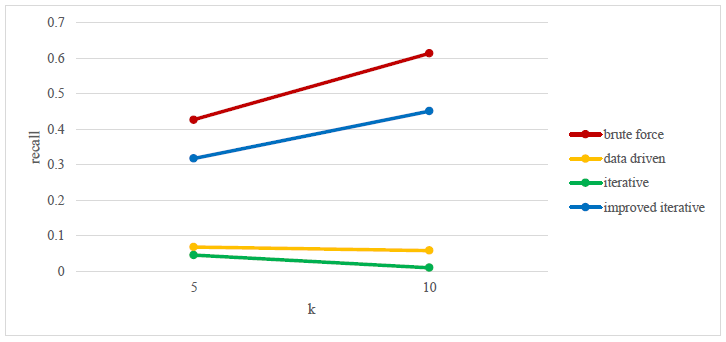
\includegraphics[width=5in]{figures/recall-of-augmented-tags-for-different-algorithms.png}
    \caption{Recall of augmented tags for different algorithms}
    \label{fig:recall-of-augmented-tags-for-different-algorithms}
\end{figure}

\begin{figure}
    \centering
    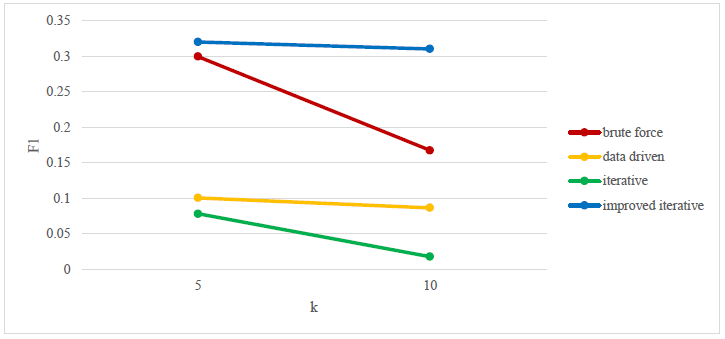
\includegraphics[width=5in]{figures/f1-of-augmented-tags-for-k-tables-in-repository.png}
    \caption{F1 of augmented tags for $k$ tables in repository}
    \label{fig:f1-of-augmented-tags-for-k-tables-in-repository}
\end{figure}

\begin{figure}
    \centering
    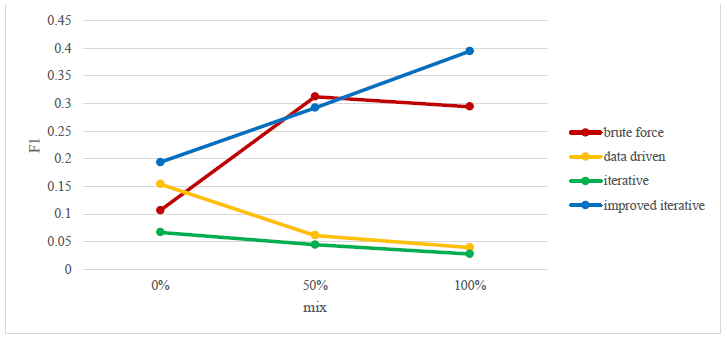
\includegraphics[width=5in]{figures/f1-of-augmented-tags-for-different-mixes-of-tables.png}
    \caption{F1 of augmented tags for different mixes of tables}
    \label{fig:f1-of-augmented-tags-for-different-mixes-of-tables}
\end{figure}

\begin{figure}
    \centering
    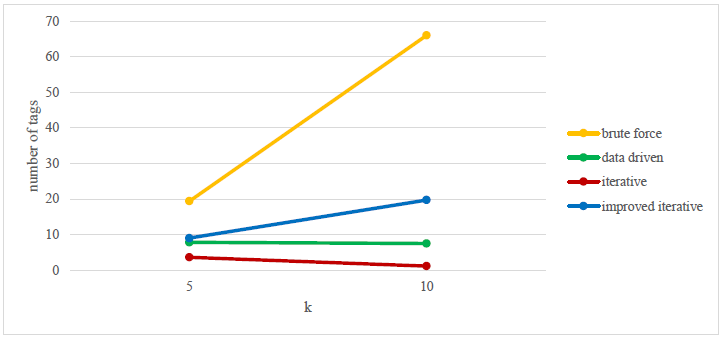
\includegraphics[width=5in]{figures/number-of-new-tags-added-given-k-tables.png}
    \caption{Number of new tags added given $k$ tables}
    \label{fig:number-of-new-tags-added-given-k-tables}
\end{figure}

\begin{figure}
    \centering
    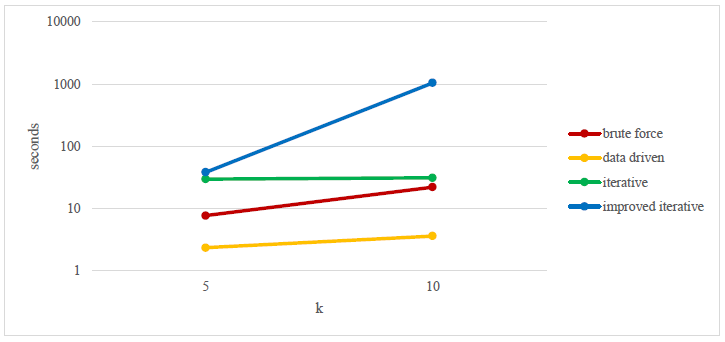
\includegraphics[width=5in]{figures/runtime-of-different-algorithms-for-different-k.png}
    \caption{Runtime of different algorithms for different $k$}
    \label{fig:runtime-of-different-algorithms-for-different-k}
\end{figure}
%%%%%%%%%%%%%%%%%%%%%%%%%%%%%%%%%%%%%%%%%%%%%%%%%%%%%%%%%%%%%%%%%%%%%%
\section{Experimental results}
\label{sec:ExperimentalResults}

We evaluate our experimental results in this section. For input repository size $k$ = 5 or 10 and with $Parks$ as the base table, we perform tests on the 4 algorithms we implemented. All tests are run on macOS 10.14 with the configuration of 1.8 GHz Intel Core i5 (5350U) and 8 GB RAM. For each repository of size $k$, we create multiple tests each with a different mix of related and unrelated tables. For example, for $k$ equal to 5, one possible mix is one base table, 2 related tables, and 2 unrelated tables. We measure the accuracy in terms of precision and recall. As a quick measure as opposed to precision and recall, we also measure the number of new tags generated regardless of the correctness of the tags. In addition to accuracy, we measure the runtime of each algorithm given a specific input. We note that each algorithm with its given input is only run once, but we would like to compute the average of multiple runs (with cross-validation) as future work.

\subsection{Precision and recall}

We measured the four algorithms in \autoref{ch:Solutions}: Solutions in terms of precision and recall with different parameters for each test. The results are shown in \autoref{tab:Precision-and-recall-of-algorithms-given-input-of-k-tables}. The accuracy of Data Driven does not reflect its actual performance, because it only creates tags for the base table and there is no mechanism for retrieving related tables. We added additional measurements for the accuracy of Improved Iterative after some modifications were made (shown in the last column of \autoref{tab:Precision-and-recall-of-algorithms-given-input-of-k-tables}). We removed the schema matching step between the attributes in the iterative method. Once a related table is found, its topics are compared to each topic in every partition. If a pair of topics has a high similarity score, the topic and the attribute are added to the partition without schema matching.

\begin{table}[ht!]
    \centering
    %\tiny
    \scriptsize
    \begin{center}
      \caption{Precision and recall of algorithms given input of $k$ tables}
      \label{tab:Precision-and-recall-of-algorithms-given-input-of-k-tables}
      %\begin{tabular}{|l|l|l|l|l|l|l|l|l|}
      % \begin{tabular}{|p{3.6em}|p{3.6em}|p{3.6em}|p{3.6em}|p{3.6em}|p{3.6em}|p{3.6em}|p{3.6em}|p{3.6em}|}  
      \begin{tabular}{|p{0.05\textwidth}|p{0.09\textwidth}|p{0.08\textwidth}|p{0.07\textwidth}|p{0.07\textwidth}|p{0.11\textwidth}|p{0.08\textwidth}|p{0.11\textwidth}|p{0.11\textwidth}|}  
        \hline
        & & & \textbf{Brute Force} & \textbf{Data Driven} & \textbf{Data Driven (base table only)} & \textbf{Iterative} & \textbf{Improved Iterative} & \textbf{Improved Iterative (additional logics removed)}\\
        \hline
        \multirow{6}{*}{k = 5} & \multirow{2}{*}{mix = 1+4} & Precision & 0.09 & 0.2 & 0.2 & 0.2857 & 0.2188 & \\
        \cline{3-9}
        & & Recall & 0.3913 & 0.1304 & 0.1304 & 0.0869 & 0.3043 & \\
        \cline{2-9}
        & \multirow{2}{*}{mix = 3+2} & Precision & 0.3625 & 0.2 &  0.2 & 0.2857 & 0.25 & \\
        \cline{3-9}
        & & Recall & 0.4203 & 0.0434 & 0.1304 & 0.0289 & 0.3623 & \\
        \cline{2-9}
        & \multirow{2}{*}{mix = 5+0} & Precision & 0.2395 & 0.1764 & 0.1764 & 0.2857 & 0.5 & \\
        \cline{3-9}
        & & Recall & 0.4693 & 0.0306 & 0.1304 & 0.0204 & 0.2857 & \\
        \hline        
        \multirow{6}{*}{k = 10} & \multirow{2}{*}{mix = 1+9} & Precision & 0.0283 & 0.1764 & 0.1764 & 0 & 0.0344 & 0.0421 \\
        \cline{3-9}
        & & Recall & 0.6956 & 0.1304 & 0.1304 & 0 & 0.5217 & 0.5217 \\
        \cline{2-9}
        & \multirow{2}{*}{mix = 5+5} & Precision & 0.0896 & 0.1667 & 0.1667 & 0.1818 & 0.2064 & 0.1042 \\
        \cline{3-9}
        & & Recall & 0.59 & 0.03 & 0.1304 & 0.02 & 0.45 & 0.42 \\
        \cline{2-9}
        & \multirow{2}{*}{mix = 10+0} & Precision & 0.1733 & 0.1667 & 0.1667 & 0.1538 & 0.4689 & 0.2059 \\
        \cline{3-9}
        & & Recall & 0.555 & 0.0137 & 0.1304 & 0.009 & 0.3807 & 0.3532 \\
        \hline
      \end{tabular}
    \end{center}
\end{table}

For every input size $k$, we took the average of the accuracy and created a plot in terms of the input size. The plot for precision is shown in \autoref{fig:precision-different-algorithms} and the plot for recall is shown in \autoref{fig:recall-of-augmented-tags-for-different-algorithms}. All four algorithms decrease in precision as the number of tables in the repository increases from 5 to 10. Data Driven decreases precision the least, from 0.19 to 0.17, while Iterative decreases the most, from 0.29 to 0.11. Improved Iterative also decreases precision, from 0.32 to 0.24, but it still has the highest precision at $k$=10 compared to the other three algorithms. However, when the additional logics are removed, the precision of Improved Iterative is only 0.11 at $k$=10, which is close to the precision of Brute Force and Iterative.

The recall either increases or decreases as $k$ increases. The recall of Iterative and Data Driven are much lower compared to the other two algorithms, and the recall of both decrease as the number of tables increases. Since the precision of Iterative and Data Driven also decrease, we consider these algorithms poorly designed. Brute Force and Improved Iterative both increase in recall as the number of tables increases, and there is a tradeoff of precision over recall as the number of tables increases. While Brute Force has the highest recall for both $k$=5 and $k$=10, the recall of Improved Iterative is comparable. We note that Brute Force has a much lower precision.

We performed roll-up of the results in the dimension of $k$, and computed the average for every mix proportion. The precision is shown in \autoref{tab:Precision-of-different-algorithms-given-a-mix-of-related-and-unrelated-tables-in-repository} and the recall is shown in \autoref{tab:Recall-of-different-algorithms-given-a-mix-of-related-and-unrelated-tables-in-repository}. A well-designed algorithm should not decrease in precision or recall when the proportion of related and unrelated tables changes. However, we observe that \textit{ImprovedIterative} decreased its precision drastically as the mix shifted from 100\% to 0\%. This suggests that Improved Iterative requires more improvements for future work.

\begin{table}[ht!]
    \centering
    \scriptsize
    \begin{center}
      \caption{Precision of different algorithms given a mix of related and unrelated tables in repository}
      \label{tab:Precision-of-different-algorithms-given-a-mix-of-related-and-unrelated-tables-in-repository}
      \begin{tabular}{|r|r|r|r|r|}
        \hline
        \textbf{mix} & \textbf{Brute Force} & \textbf{Data Driven} & \textbf{Iterative} & \textbf{Improved Iterative} \\
        \hline
        0\% & 0.05915 & 0.1882 & 0.14285 & 0.1266 \\
        \hline
        50\% & 0.22605 & 0.18335 & 0.23375 & 0.2282 \\
        \hline
        100\% & 0.2064 & 0.17155 & 0.21975 & 0.48445 \\
        \hline
      \end{tabular}
    \end{center}
\end{table}

\begin{table}[ht!]
    \centering
    \scriptsize
    \begin{center}
      \caption{Recall of different algorithms given a mix of related and unrelated tables in repository}
      \label{tab:Recall-of-different-algorithms-given-a-mix-of-related-and-unrelated-tables-in-repository}
      \begin{tabular}{|r|r|r|r|r|}
        \hline
        \textbf{mix} & \textbf{Brute Force} & \textbf{Data Driven} & \textbf{Iterative} & \textbf{Improved Iterative} \\
        \hline
        0\% & 0.54345 & 0.1304 & 0.04345 & 0.413 \\
        \hline
        50\% & 0.50515 & 0.0367 & 0.02445 & 0.40615 \\
        \hline
        100\% & 0.51215 & 0.02215 & 0.0147 & 0.3332 \\
        \hline        
      \end{tabular}
    \end{center}
\end{table}

We then performed roll-up of the results in both $k$ and mix proportion. Improved Iterative has the highest precision of 0.28 while Brute Force has the lowest precision of 0.16, but Brute Force has the highest recall of 0.52 while Iterative has the lowest recall of 0.03. We think that Brute Force has a high recall because it blindly adds all tags it finds. The reason that Iterative has a low recall is because it only uses N-gram as the matching criterion, which fails to identify semantically similar tags.

We ranked the four algorithms based on how well they performed for each test. Of the 12 tests, Improved Iterative ranks first 7 times and ranks second 3 times. The only test it performs much worse than another algorithm is for $k$=10, and the repository contains 9 unrelated tables. We think Improved Iterative cannot correctly reject unrelated tables, and therefore adds too many incorrect tags. The semantic distance is affected by the initialization step, which we may need to improve in the future.

Using the precision and recall, we now compute the F1 score for the four algorithms. The plot for the F1 score at different $k$ is shown in \autoref{fig:f1-of-augmented-tags-for-k-tables-in-repository}. The plot for the F1 score for different mix proportions of related and unrelated tables is shown in \autoref{fig:f1-of-augmented-tags-for-different-mixes-of-tables}.

As $k$ increases, the F1 score for all of the algorithms decreases, but different algorithms decrease at different magnitudes. The F1 score for Brute Force decreases the most, from 0.30 to 0.17, while Improved Iterative decreases the least, from 0.32 to 0.31. Improved Iterative performs the best for all $k$. As the mix proportion changes, F1 for each of the four algorithms changes in different ways. Data Driven and Iterative decrease in F1 as the mix proportion increases, while Improved Iterative increases in F1 as the mix proportion increases. Brute Forces F1 increases at 50\% but decreases at 100\%. Improved Iterative performs the best among all four algorithms.

However, we think a good algorithm should have a constant F1 score regardless of what mix proportion it is given. This suggests again that more improvements need to be done as future work.

\subsection{New tags added}

We measured the number of new tags added to the augmented metadata for the four algorithms in \autoref{tab:Number-of-new-tags-added-by-different-algorithms}. Brute Force adds the greatest number of new tags on average, 42.71 per table, Data Driven adds 7.63 tags per table, while Iterative only adds 2.33 per table. Improved Iterative adds 14.35 tags per table. When additional logics are removed for Improved Iterative, 25.96 new tags are added. This demonstrates that the schema matching step is able to filter out many tags.

\begin{table}[ht!]
    \centering
    \scriptsize
    \begin{center}
      \caption{Number of new tags added by different algorithms}
      \label{tab:Number-of-new-tags-added-by-different-algorithms}
      \begin{tabular}{|p{0.05\textwidth}|p{0.14\textwidth}|p{0.08\textwidth}|p{0.07\textwidth}|p{0.07\textwidth}|p{0.11\textwidth}|p{0.14\textwidth}|}  
        \hline
         & & \textbf{Brute Force} & \textbf{Data Driven} & \textbf{Iterative} & \textbf{Improved Iterative} & \textbf{Improved Iterative (additional logics removed)}\\
        \hline
        \multirow{3}{*}{k = 5} & mix = 1+4 & 17 & 15 & 7 & 6 & \\
        \cline{2-7}
        & mix = 3+2 & 14.67 & 5 & 2.33 & 13 & \\
        \cline{2-7}
        & mix = 5+0 & 26.4 & 3.4 & 1.4 & 8 & \\
        \hline        
        \multirow{3}{*}{k = 10} & mix = 1+9 & 63 & 17 & 0 & 29 & 41 \\
        \cline{2-7}
        & mix = 5+5 & 70.2 & 3.6 & 2 & 16.2 & 20.4 \\
        \cline{2-7}
        & mix = 10+0 & 65 & 1.8 & 1.3 & 13.9 & 16.5 \\
        \hline
      \end{tabular}
    \end{center}
\end{table}

Since Brute Force adds every tag from a related table, we can compare other algorithms with Brute Force to estimate the selectivity of the other algorithms. Iterative is highly selective, since there are no new tags added for the test $mix = 1+9$, either because no related tables are found or none of the tags in the related tables are similar to the base table tags. This outcome is desirable because none of the 9 tables in the repository are related to the base table. Data Driven does not add many new tags either, since there is an upper bound on the number of new tags, which equals to the number of attributes in the base table. Improved Iterative adds more new tags than Data Driven, but less than Brute Force.

The plot in \autoref{fig:number-of-new-tags-added-given-k-tables} shows the average number of tags added as $k$ increases. For Brute Force, the number of tags added per table increases as expected, since there is one or more tags per table on average. For Data Driven, the number of new tags does not change, since the number of attributes in the base table remains constant. For Iterative, as repository size increases, the number of new tags added per table decreases. This is due to the uncontrollable factor that we have different tables between the testing set for $k$ = 5 and $k$ = 10. There are more new tags that Iterative can add for the $k$ = 5 set and there are less that it can add for the $k$ = 10 set. For Improved Iterative, the number of new tags doubles as $k$ doubles, which is a desired result.

\subsection{Runtime}
We measured the runtime for the four different algorithms, and the results are shown in \autoref{tab:Runtime-of-different-approaches-given-k-tables-as-input}. Each test can be completed within a reasonable timeframe for all of the algorithms. Iterative and Improved Iterative terminated the iterative method in less than 5 iterations (either $2^{nd}$, $3^{rd}$, or the $4^{th}$ iteration) for all tests. However, we have not included any tests with more than 10 tables in the repository, and we cannot conclude that any of the algorithms is efficient.

\begin{table}[ht!]
    \centering
    \scriptsize
    \begin{center}
      \caption{Runtime (in seconds) of different approaches given $k$ tables as input}
      \label{tab:Runtime-of-different-approaches-given-k-tables-as-input}
      \begin{tabular}{|p{0.05\textwidth}|p{0.14\textwidth}|p{0.08\textwidth}|p{0.07\textwidth}|p{0.07\textwidth}|p{0.11\textwidth}|p{0.14\textwidth}|}  
        \hline
         & & \textbf{Brute Force} & \textbf{Data Driven} & \textbf{Iterative} & \textbf{Improved Iterative} & \textbf{Improved Iterative (additional logics removed)}\\
        \hline
        \multirow{3}{*}{k = 5} & mix = 1+4 & 1.2 & 0.76 & 12.41 & 6.12 & \\
        \cline{2-7}
        & mix = 3+2 & 2.24 & 0.77 & 7.06 & 25.16 & \\
        \cline{2-7}
        & mix = 5+0 & 4.21 & 0.8 & 10.05 & 6.7 & \\
        \hline        
        \multirow{3}{*}{k = 10} & mix = 1+9 & 8.02 & 1.31 & 10 & 268 & 13 \\
        \cline{2-7}
        & mix = 5+5 & 5.63 & 1.19 & 9 & 135 & 4 \\
        \cline{2-7}
        & mix = 10+0 & 8.23 & 1.07 & 12 & 639 & 5 \\
        \hline
      \end{tabular}
    \end{center}
\end{table}

We created a plot to show the runtime of each algorithm as the repository size $k$ increases, shown in \autoref{fig:runtime-of-different-algorithms-for-different-k}. Each value is an average of three tests of different mixes of related and unrelated tables. We observe that Brute Force, Data Driven, and Iterative do not increase in runtime by orders of magnitude, but Improved Iterative increases from 38 seconds to 1,042 seconds as $k$ increases from 5 to 10. Empirically, it is likely that the algorithm has exponential asymptotic complexity. We measured the time to enrich attributes and topics of each table in the repository, and the time to enrich 5 tables is around 3 seconds. We also measured the time to perform semantic labeling between attributes and tags: the time is around 15 seconds for 5 tables. Most of the computation time is in the schema matching step in the iterative method. As we removed the additional logics, the runtime drops significantly and the runtime of Improved Iterative is comparable to the Iterative.

We analyzed the theoretical asymptotic upper bound for the iterative method. For $n$ tables, $t$ tags per table, $m$ attributes per table, and assuming the matching criterion make comparisons in $O(1)$, the upper bound of the iterative method is approximately $nt(nt*nt+t*nt*(nt+nm))$, or $O(n^3t^4+n^3t^3m)$. The maximum number of iterations is $nt$ since we add at least one tag to the base table partitions per iteration and will not consider that tag again in future iterations. For each iteration, the table search step makes at most $nt*nt$ tag comparisons. Once a related table is found, the partitioning step for the semantic labels is $t*nt*(nt+nm)$, since there are $t$ candidate tags, $nt$ partitions, and within each partition there are $nt$ tags and $nm$ attributes. Based on the theoretical bound, the iterative method has polynomial complexity.

We removed the schema matching step on the attributes that may have contributed to the increase in runtime, and the complexity of the iterative method is reduced to $O(n^3t^3)$.
\endinput